\documentclass[12 pt]{article}
\usepackage{fancyhdr}
\usepackage[margin = 1 in]{geometry}
\usepackage{amsmath}
\usepackage{enumerate}
% \usepackage{indentfirst}
\pagestyle{fancy}
\usepackage{graphicx}
\usepackage[version=3]{mhchem}
\fancyhf{}
\usepackage{sectsty}	
\lhead{Andrew Wang}
\chead{CS/CNS/EE 155 Machine Learning \& Data Mining}
\rhead{Yue}
\sectionfont{\fontsize{15}{18}\selectfont}
\usepackage{graphicx}
\usepackage{array}
\newcolumntype{P}[1]{>{\centering\arraybackslash}p{#1}}
\newcolumntype{M}[1]{>{\centering\arraybackslash}m{#1}}
\usepackage[font=small,labelfont=bf]{caption}
\usepackage{float}
\usepackage{float}
\usepackage{subfig}
\usepackage{microtype}
\usepackage{ amssymb }
\usepackage{amsmath}
\usepackage{commath}
\begin{document}
	\begin{center}
		\section*{Homework 6}
	\end{center}
	
	
	\subsection*{1 SVD and PCA}	
	\noindent\textbf{Question A:}  \\
	If $Y = X^T$ and SVD of $Y = U \Sigma V^T$ then  $X=Y^T$ and $X = $ ${(U \Sigma V^T)}^T = V \Sigma U^T$. Now we have:
	
	\[ X X^T = V \Sigma U^T U \Sigma V^T\]
	\[       = V \Sigma^2 V^T \]
	
	\noindent If we perform PCA on X, we diagonalize $XX^T$ i.e. find $U$ and $\Lambda$ such that $XX^T = U \Lambda U^T$. In this case, we see that this $U$ is $V$, $\Lambda = \Sigma ^2$ and so the columns of $V$ are the principal components of $X$. \\
	
	
	\noindent\textbf{Question B:}  \\
	We seek to prove that SVD is the best rank at-most-k approximation in the Frobenius norm. 
	
	\[A_k = argmin_{rank(B)\leq k} \norm {A - B}_F = argmin_{rank(B)\leq k} \norm {U \Sigma V^T - B}_F \]
	
	\noindent Converting this by multiplying by an orthogonal matrix that keeps the Frobenious Norm the same and which does not change the rank of the matrix, we get :
	
 	\[ argmin_{rank(B)\leq k} \norm {\Sigma - U^T B V}_F \]
 	
 	\noindent Going off the Piazza post, we know that to minimize $\norm {\Sigma - U^T B V}_F$, $U^TBV$ should be a diagonal matrix with the first $k$ elements of the diagonal of $\Sigma$ and other diagonal elements 0 because adding off-diagonal elements to $U^TBV$ will not help minimize $\norm {\Sigma - U^T B V}_F$, $U^TBV$. In other words, we minimized:
 	
 	\[ \sum_{i}(\Sigma_{i,i} - D_{i,i})^2  \]
 	
 	\noindent where $D = U^TBV$. This implies $UDV^T = B$ and thus we get that $A_k = \sum_{j = 1}^{k} u_j\sigma_jv_j^T = \sum_{j = 1}^{k} \sigma_ju_jv_j^T$.

	
	\subsection*{2 Matrix Factorization}
	\noindent\textbf{Question A:} \\
	\[\partial_{u_i} = \lambda u_i - \sum_{j}v_j (y_{ij} - u_i^Tv_j)\]
	\[\partial_{v_j} = \lambda v_j - \sum_{i}u_i (y_{ij} - u_i^Tv_j)\]
	\noindent\textbf{Question B:} \\
	Setting $\partial_{u_i} = 0$ and $\partial_{v_j} = 0$ to find critical points of our regularized square error , we get the following:
	
	\[0 = \partial_{u_i} = \lambda u_i - \sum_{j}v_j (y_{ij} - u_i^Tv_j)\]
	
	\[0 = \lambda u_i - \sum_{j}v_j y_{ij} + \sum_{j} v_j u_i^Tv_j\]
	
	\[0 = \lambda u_i - \sum_{j}v_j y_{ij} + \sum_{j} v_j v_j^T u_i\]
	
	\[0 = \lambda u_i - \sum_{j}v_j y_{ij} +  (\sum_{j} v_j v_j^T)u_i\]
	
	\[\sum_{j}v_j y_{ij} = \lambda u_i  + (\sum_{j} v_j v_j^T)u_i \]
	
	\[\sum_{j}v_j y_{ij} = (\lambda I +  \sum_{j} v_j v_j^T) u_i\]
	
	\[(\lambda I +  \sum_{j} v_j v_j^T)^{-1} \sum_{j}v_j y_{ij} = u_i\]
	
	Similarly, for $\partial_{v_j}$: 
	
	\[0 = \partial_{v_j} = \lambda v_j - \sum_{i}u_i (y_{ij} - u_i^Tv_j)\]
	
	\[0 = \lambda v_j - \sum_{i}u_i y_{ij} + \sum_{i} u_i u_i^Tv_j\]
	
	
	\[0 = \lambda v_j - \sum_{i} u_i y_{ij} +  (\sum_{i}  u_i  u_i^T)v_j\]
	
	\[\sum_{i} u_i y_{ij} = \lambda v_j  + (\sum_{i}  u_i u_i^T)v_j \]
	
	\[\sum_{i} u_i y_{ij} = (\lambda I +  \sum_{i}  u_i  u_i^T) v_j\]
	
	\[(\lambda I +  \sum_{i}  u_i  u_i^T)^{-1} \sum_{i}u_i y_{ij} = v_j\]
	
	
	
	

	%\begin{figure}[h]
	%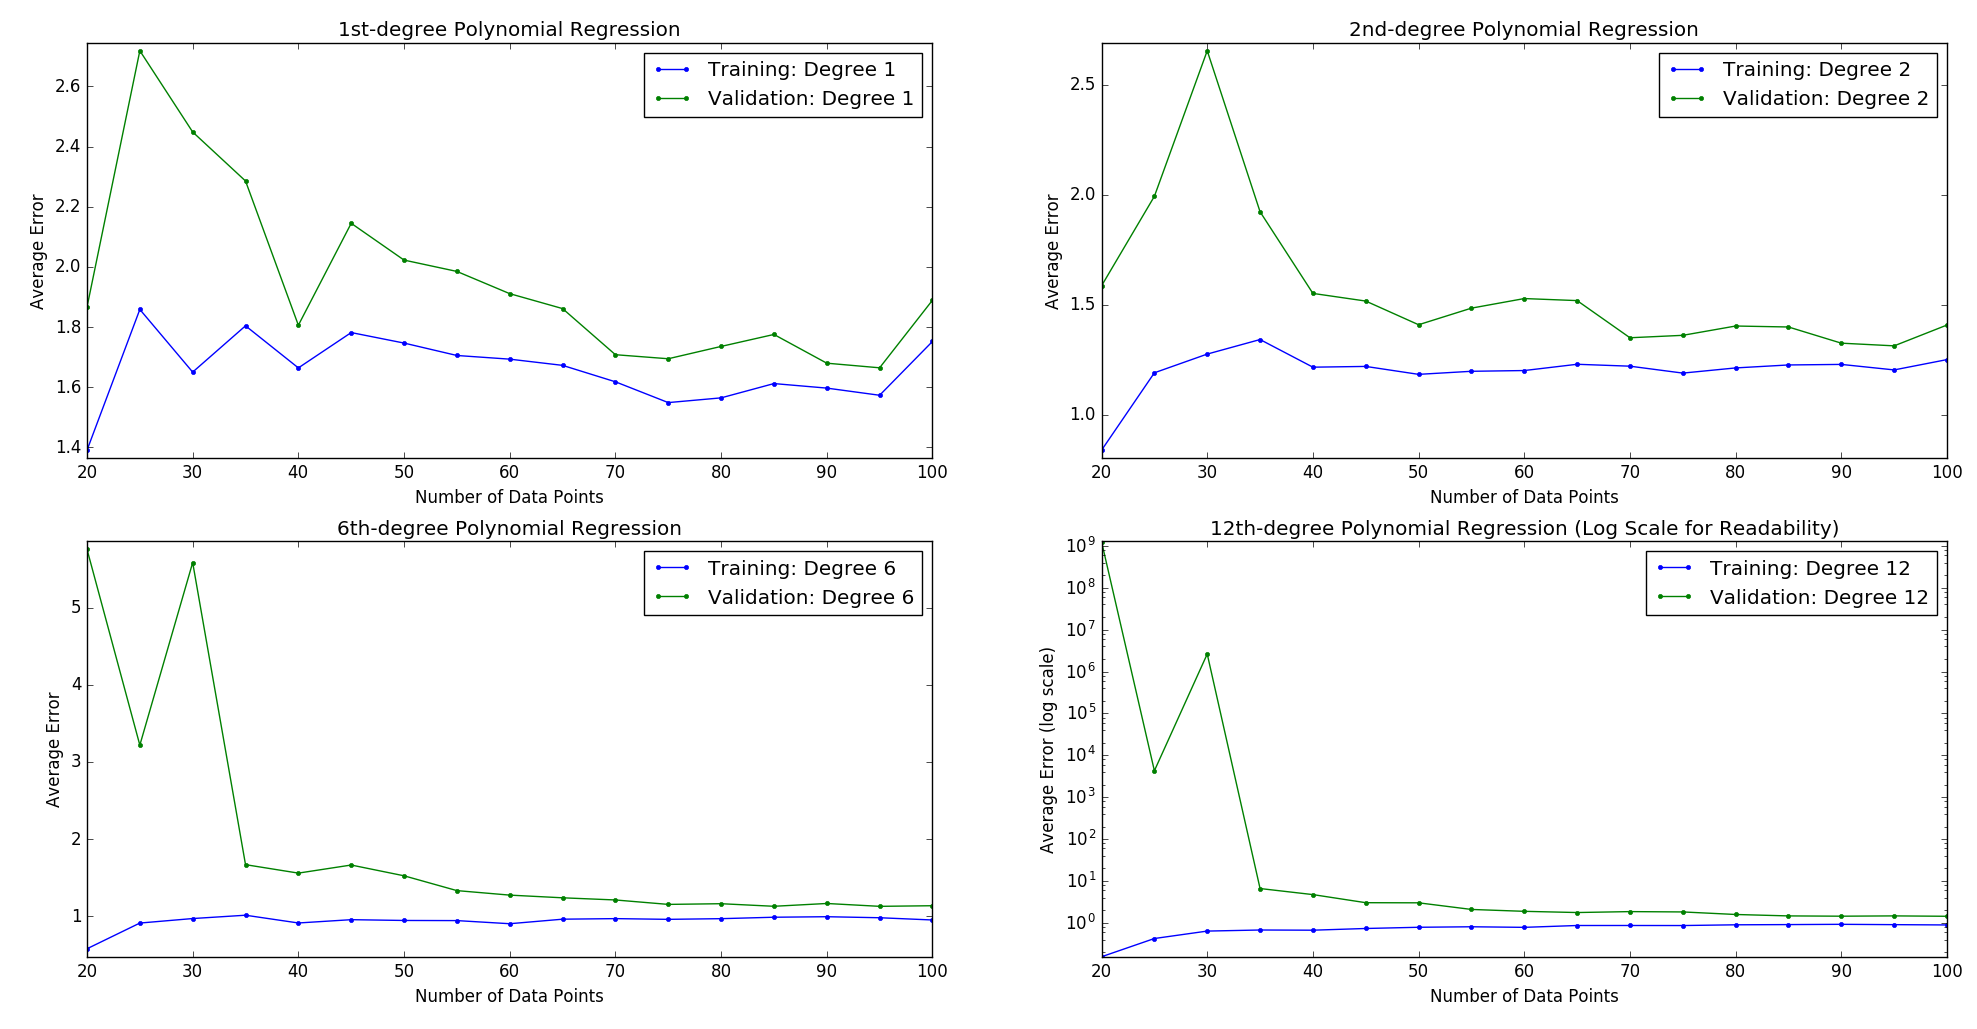
\includegraphics[width=17cm]{LearningCurves}
	%\end{figure}	
	
	\noindent\textbf{Question C:}  \\
	See attached code. \\
	
	\noindent\textbf{Question D:} \\
	\begin{figure}[H]
	\centering
	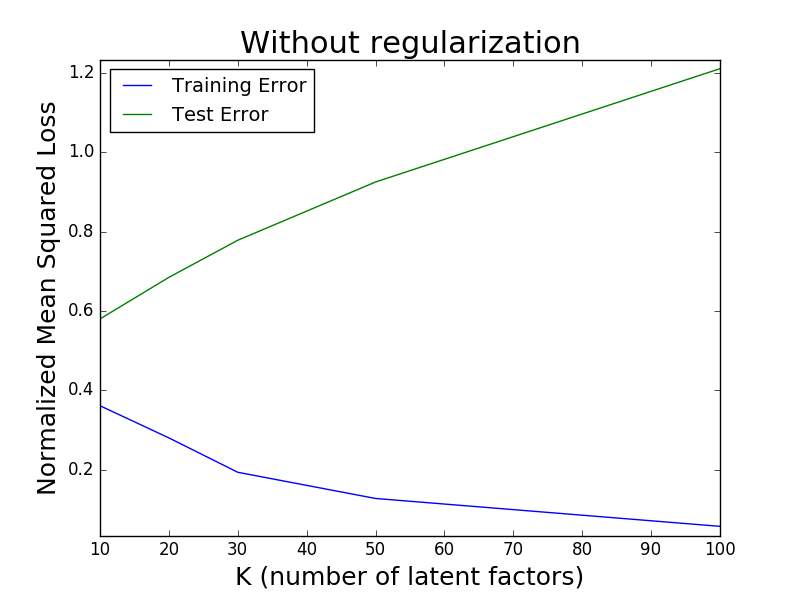
\includegraphics[width=\textwidth]{2D}
	\caption{E$_{in}$ and E$_{out}$ vs. k with $\lambda = 0$}
	\end{figure}
	
	\noindent We observe that as $k$ increases, E$_{in}$ decreases while E$_{out}$ increases. We know that $k$, the number of latent factors, determines the level of dimensionality reduction such that a small $k$ represents small matrices $U$ and $V$ and therefore a large reduction in dimensionality of our original input space. In these terms, the more we lower $k$ and the more we reduce the dimensions of the input space, the more we are summarizing the original data. This summarization can prevent the model from overfitting to the training set because in summarizing the input data, it is not fitting to the peculiarities of the data itself. Thus, we see that for low $k$ where we summarize the input data the most, we have low $E_{out}$ and high $E_{in}$ and as we increase k, we are getting more likely to overfit to the training input data, so E$_{in}$ goes down at the cost of generalization where E$_{out}$ increases. \\

	
	\noindent\textbf{Question E:} \\
	
	\begin{figure}[H]
		\centering
		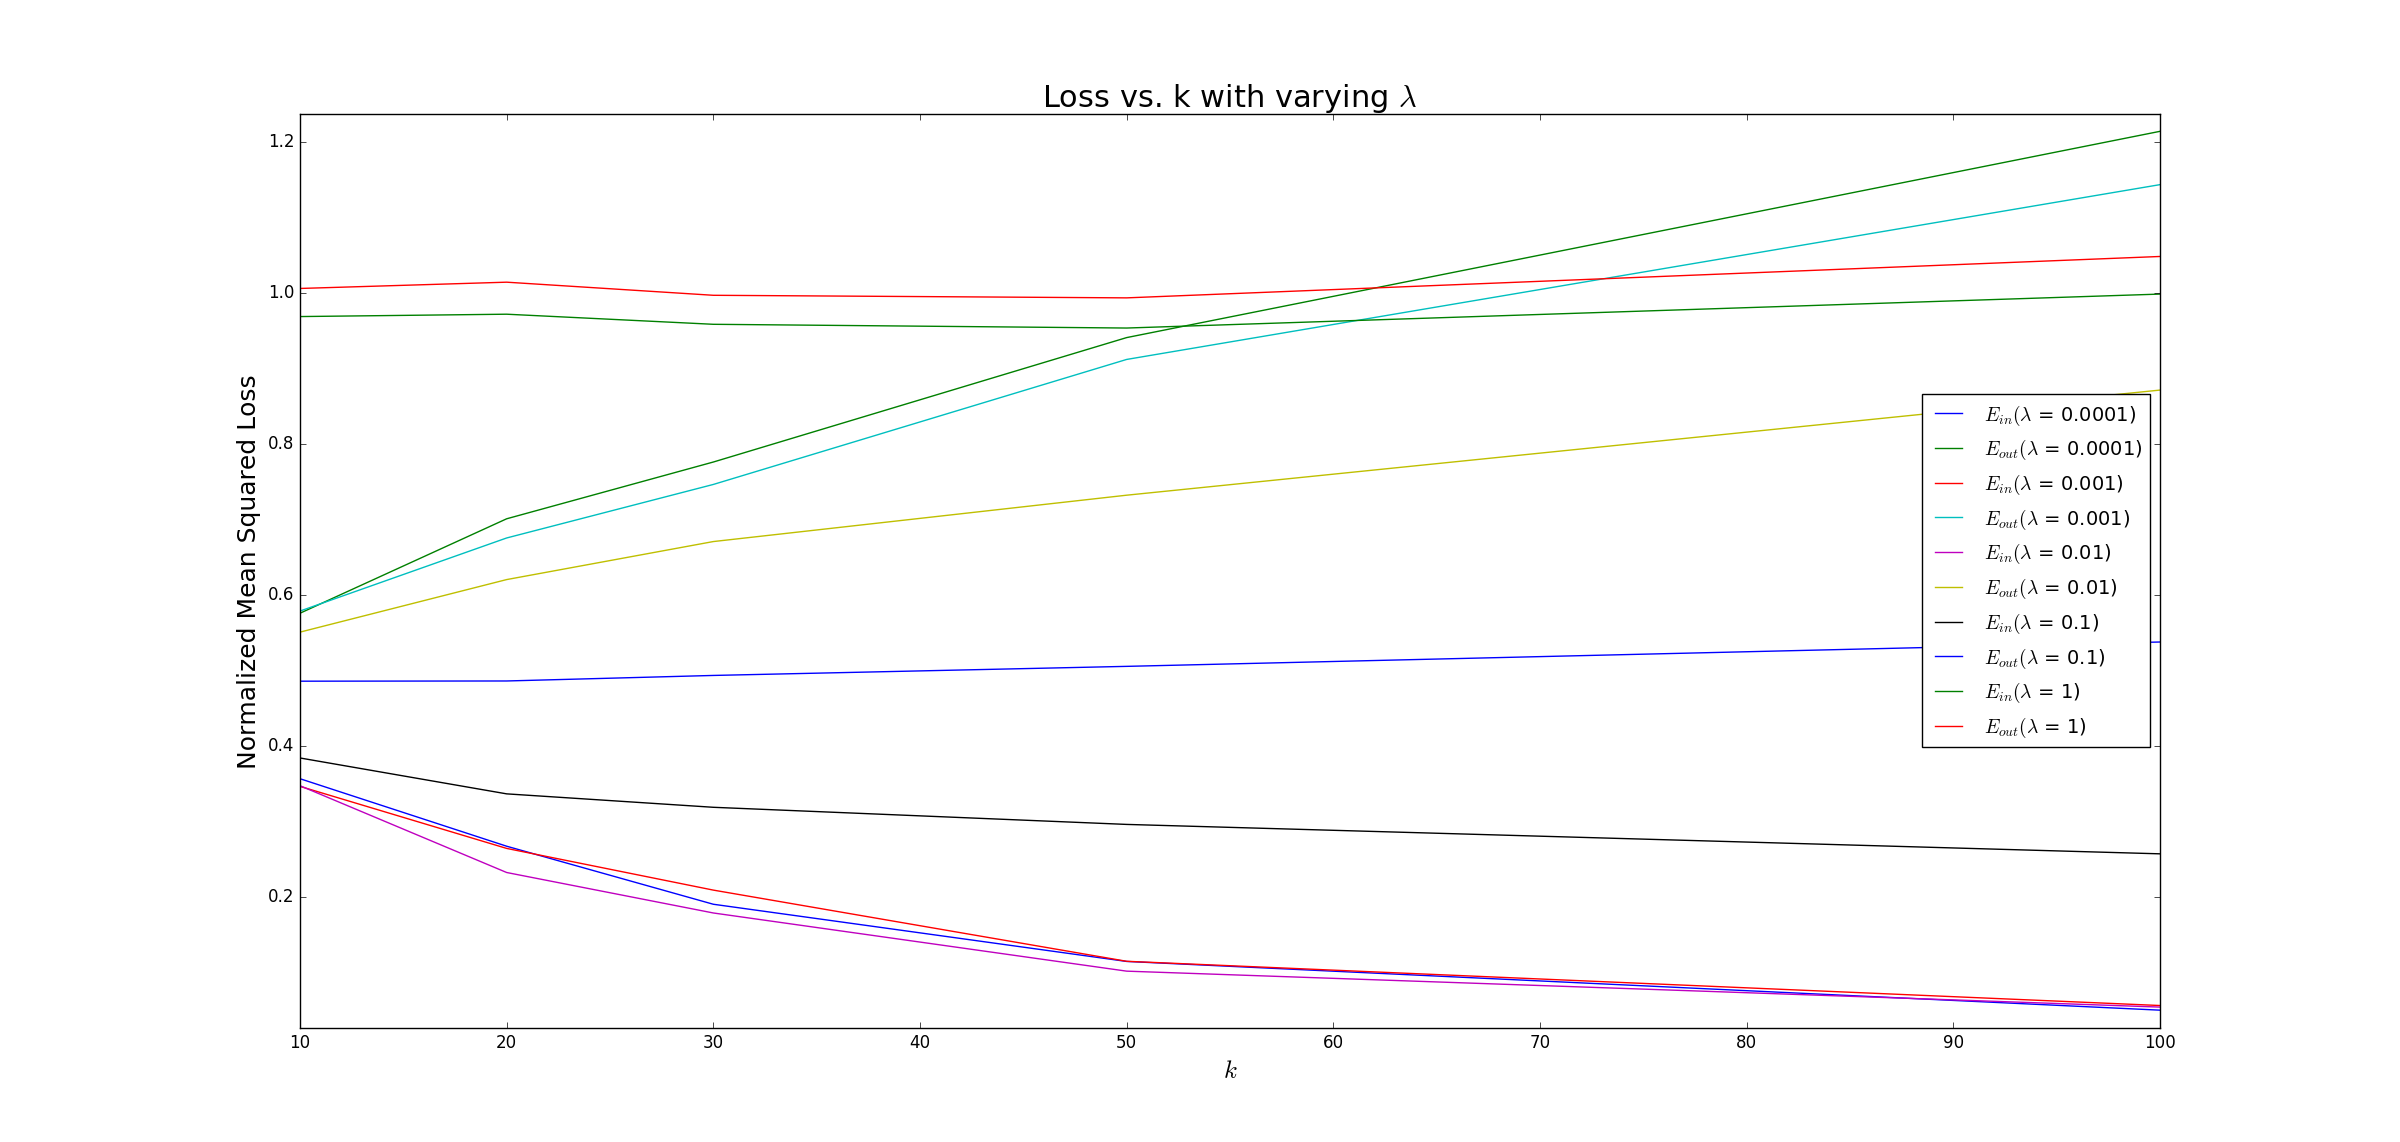
\includegraphics[width=\textwidth]{LossVsK}
		\caption{E$_{in}$ and E$_{out}$ for $k$ = 10, 20, 30, 50, 100 for each  $\lambda$ = 0.0001, 0.001, 0.01, 0.1, 1}
	\end{figure}

	\noindent We observe similar trends to the previous graph where increasing k typically decreases E$_{in}$ and increase E$_{out}$. When $\lambda$ is too large, such as when $\lambda = 1$, we see that we have high $E_{in}$ and $E_{out}$, a sign of underfitting. As we decrease $\lambda$, the closer the results resemble that of the previous graph where $\lambda = 0$. Out of the five values for $\lambda$, the best results seem to come from when $\lambda = 0.1$ where we have the lowest E$_{out}$. At $\lambda = 0.1$, we seem to combat both underfitting and overfitting.  
	
	

	\begin{figure}[H]
	\centering
	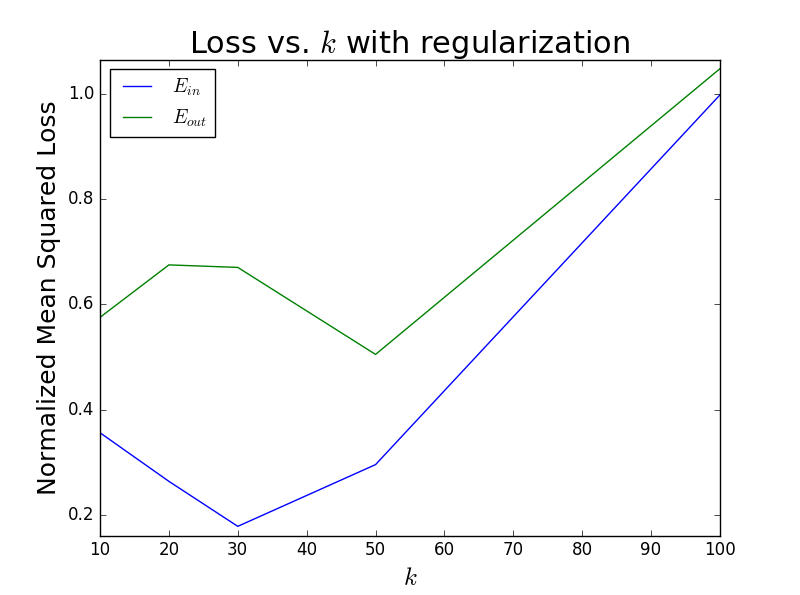
\includegraphics[width=13cm]{2E_singleGraph}
	\caption{E$_{in}$ and E$_{out}$ for $k$ = 10, 20, 30, 50, 100 for  $\lambda$ = 0.0001, 0.001, 0.01, 0.1, 1 respectively (as mentioned in Piazza post). Not sure if this graph is required, but just added in case.}
	\end{figure}
	

	
	\subsection*{3 Word2Vec Principles}
	\noindent\textbf{Question A:} \\
	\noindent We have: $log \; p(w_O |w_I) = log \dfrac{exp(v_{w_O}^{'T}v_{w_I})}{\sum_{w = 1 }^{W} exp(v_w^{'T}v_{W_I})}$. \\ 
	
	\noindent Computing $\nabla \;log \; p(w_O |w_I)$ scales linearly with $W$. First off, we note that computing the derivative of the numerator takes constant time. Now, we analyze the denominator of $p(w_O | w_I)$ and observe that as we increase $W$, we increase the number of terms in the summation for the denominator. Each time we increase $W$ by 1, then we have 1 more additional term to differentiate in the denominator.  Thus, computing $\nabla \;log \; p(w_O |w_I)$ is O($W$). \\
	
	\noindent\textbf{Question B:} \\
	\noindent Because $p(w_O |w_I)$ involves multiplying $v^T$ and $v$ and $v \epsilon R^D$, as we increase D, we also increase the computational complexity of computing the training objective. For large D, it may be very computationally intensive to carry out such calculations. In addition, as we increase D, we are more likely to overfit to the training set, potentially generalizing poorly. This is indeed undesirable. \\
	
	\noindent\textbf{Question C:} \\ See attached code. \\
	
	\noindent\textbf{Question D:} \\ 
	\textbf{i.} Dimensions of weight matrix of hidden layer: 311 x 10. \\
	\textbf{ii.} Dimensions of weight matrix of output layer: 10 x 311. \\
	\textbf{iii.}
	\begin{figure}[H]
		\centering
		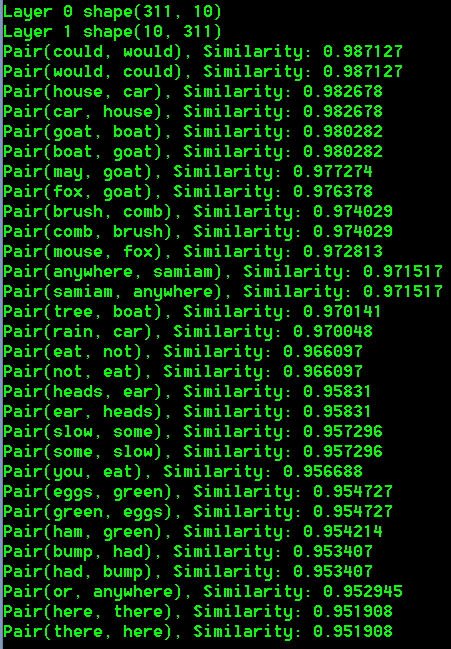
\includegraphics[width=10cm]{Pairs}
		\caption{Top 30 pairs of most similar words}
	\end{figure}
	\noindent I noticed that we have many repeats where Pair(a,b) and Pair(b,a) are both included. This makes sense given that if word a is often seen with word b, then word b is often seen with word a. If we look at these pairs, many of the pairing words make up well-known Dr. Seuss phrases.  For example, we have the pairs (``ham", ``green") and (``eggs", ``green") which are words used in the famous phrase ``green eggs and ham."  Other examples include the pair (``here", ``there") as the phrase ``here and there" is repeated many times in Dr. Seuss' poems. Another common theme between these top similar pairs are that the words rhyme such as in (``could", ``would") and (``goat, boat"). This also makes sense given that Dr. Seuss wrote poems that have a repetitive rhyming scheme such that words that rhyme are typically neighbored by the similar words. Additionally, many of these pairs consist of two of the same type of objects such as two animals or two body parts. \\
	
	\noindent\textbf{Question E:} \\
	To calculate the expected frequency of a word $w_i$ after subsampling, we simply subtract the number of times we expect to discard the word from $f(w_i)$, the frequency of the word. This is formulated as:
	
	\[ \mathbb{E}[f(w_i)] = f(w_i) - P(w_i) f(w_i) \]
	\[                    = f(w_i) (1 - P(w_i))\]
	\[                       = f(w_i)(1 - (1 - \sqrt{\frac{t}{f_{w_i}}}))\]
	\[                        = f(w_i)\sqrt{\frac{t}{f_{w_i}}} \]
	\[ = \sqrt{tf(w_i)} \]
	
	\noindent Because t is a constant, we have that if $f(w_i) > f(w_j)$ before subsampling, then $\sqrt{tf(w_i)} > \sqrt{tf(w_j)}$. Therefore $\mathbb{E}[f(w_i)] > \mathbb{E}[f(w_j)]$ after subsampling and thus ranking of frequencies is preserved in expectation by the subsampling policy. 
	
	
\end{document}